\section{Excercise 9}
Cho mạch sau. Tìm điện áp \(v\) và dòng điện \(i_x\) . Theo kết quả, xác định các linh kiện có khả năng hấp thụ lần lượt là p1 và p2 là hoạt động hoặc
thụ động (cần tính toán). Lưu ý rằng ở đây chúng tôi sử dụng quy ước ký hiệu thụ động.
Nếu một phần tử tiêu thụ điện năng, hãy sử dụng điện trở thuần có giá trị phù hợp làm đại diện. Nếu là bộ phận cấp nguồn, hãy sử dụng nguồn điện áp DC lý tưởng tương ứng để
đại diện cho nó. Thực hiện mô phỏng để kiểm tra mạch hoạt động như thế nào.
\begin{figure}[!htbp]
    \centering
    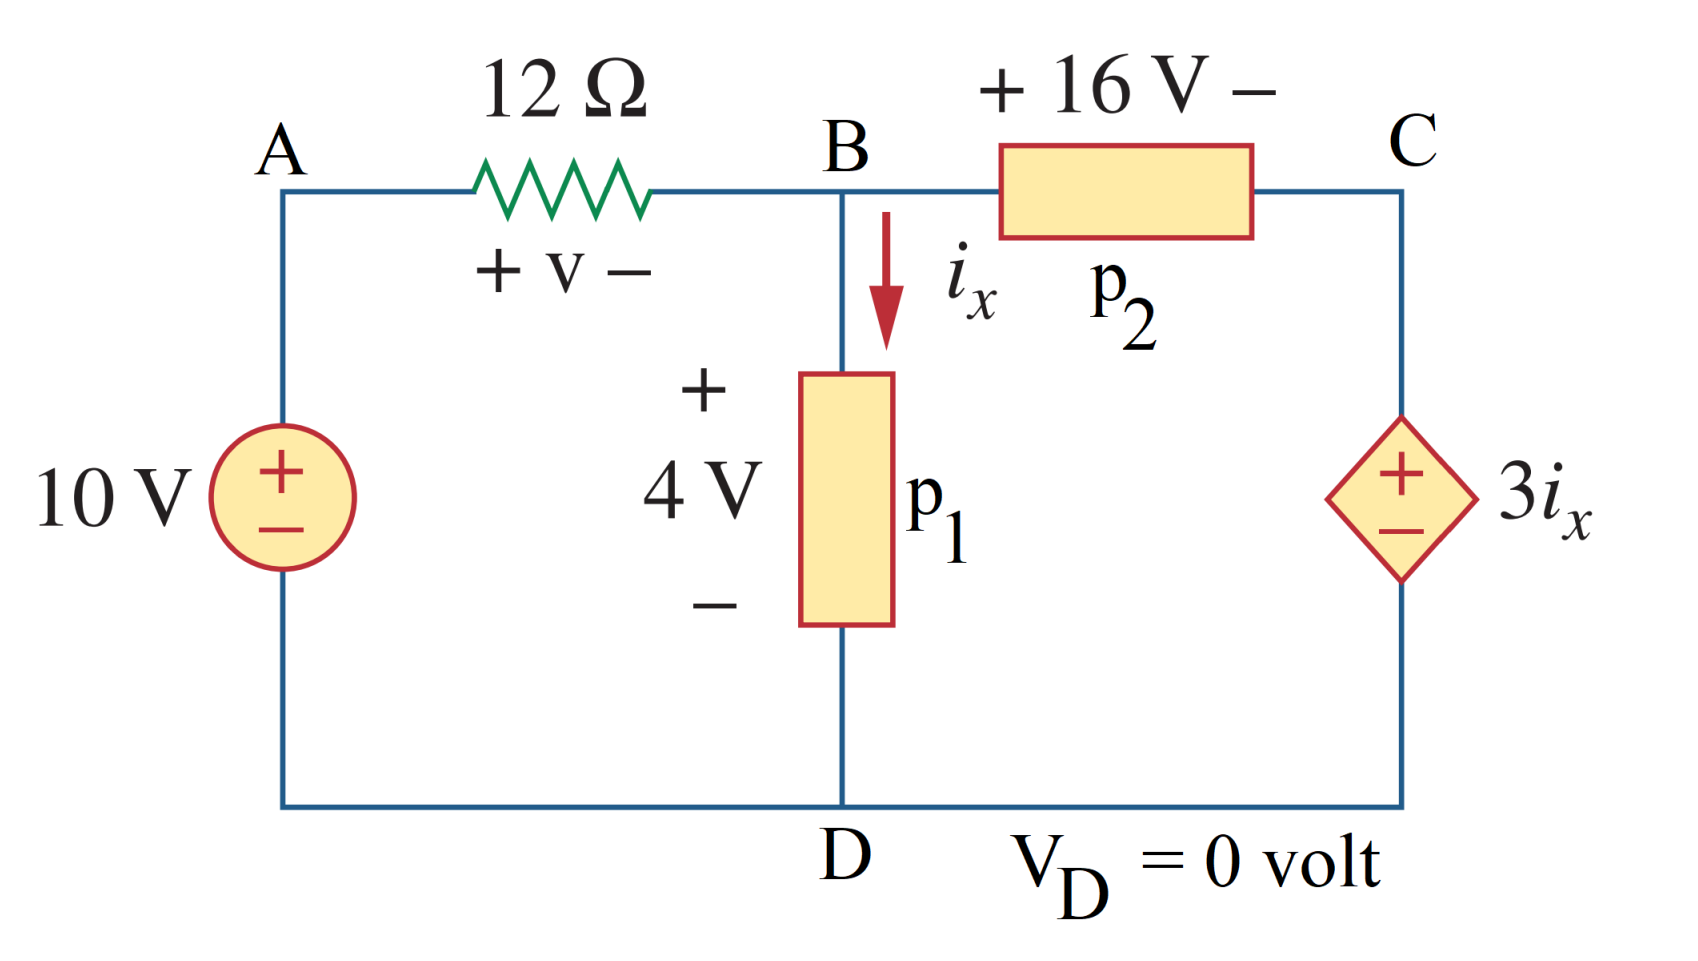
\includegraphics[width=0.7\textwidth]{graphics/ex9/f1.png}
    \caption{Tìm các phần tử và biến chưa biết, sau đó kiểm tra chúng bằng mô phỏng}
    \end{figure}
\subsection{Tính toán}
\textbf{Ghi chú:}
Giải thích, công thức và phương trình được mong đợi hơn là chỉ có kết quả.\\
Theo phân tích lưới.\\
Vòng 1:
\begin{align*}
12I_{AB} + 4 - 10 = 0 \rightarrow I_{AB} = 0,5 (A).
\end{align*}
Vòng 2:
\begin{align*}
    -4 + 16 + 3i_x = 0 \rightarrow i_x = -4 (A).
\end{align*}
Ta có:
\begin{align*}
    v = I_AB.12 =6 (V)\\
    i_x = -4 (A).
\end{align*}
